% Generated by scripts/2026-10-21/extract_floats.py from paper/main_ko.tex; edit the full manuscript, not this file.
\begin{figure}[htbp]
\centering
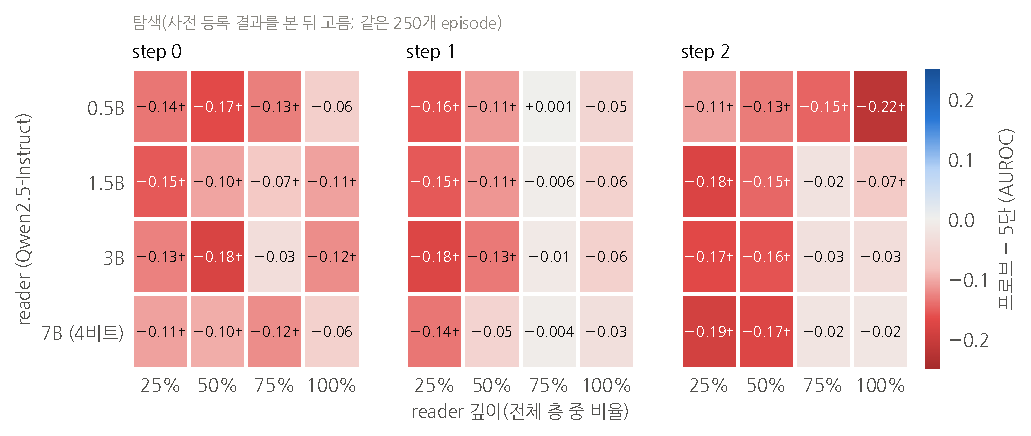
\includegraphics[width=\linewidth]{fig4_reader_depth_ko.pdf}
\caption{탐색: 처음 250 episode에서 선형 프로브의 모든 reader $\times$ 깊이 조합의 프로브 $-$ 5단 AUROC 차이(48칸, 선택 없음). 0을 중심으로 한 발산 색(빨강: 프로브가 5단보다 낮음). $\dagger$는 95\% CI(scene 단위 군집 bootstrap)가 0을 포함하지 않는 칸이며 모두 0 아래다(48칸 중 31칸). CI가 0 위에 있는 칸은 없고 가장 큰 차이는 $+0.001$이다. 7B reader는 4비트 가중치를 써서 크기와 양자화가 섞여 있다. MLP 칸과 CI: 부록 표~\ref{tab:a6}.}\label{fig:heat}
% 출처: results/explore_{0.5B,1.5B,3B,7B-4bit}_diff.csv
\end{figure}
